\documentclass{article}
\usepackage{hyperref}
\usepackage[margin=1in]{geometry}
\usepackage{graphicx}
\graphicspath{{./img/}}

\begin{document}
\title{\vspace{-2cm}Research Paper Outline}
\author{Armant Touche}
\maketitle

\section{Intro}

    \subsection{Thesis} Thesis: $(1/4) - (1/3)$ of paper The purpose of my research is to prove that humans' activities contribute to streamflow change and to quantify how human much contribute (i.e. man-made water structure, agriculture, and other yet to be stated).

    \subsection{Support}
    \begin{enumerate}
        \item Describe the "human disturbance" index from Falcone 2016 and it's accuracy is dependent on GIS tricky implementation:
            \begin{enumerate}
                \item GIS implementation
                \item The six variables from the reduced variable index: HUDEN, ROADDEN, PESTIC, URBCP\_MAINS, DIST\_CANAL\_NEAR and DAMSTOR. 
                \item resulting accuracy of previously indexed watershed classification from USEPA (pg. 269)
            \end{enumerate}

        \item Implmentaion of the "human distrubance" index from Falcone 2016 in the Rice 2016 study
            \begin{enumerate}
                \item State 70 annual scale streamflow dataset (1940 - 2009) and show the correlation amongst the ecoregions with figure 1
                \item State the two variables that were considered important in hinting at a conclusive answer $P_\textit{mean} \;\&\; {DI}_\textit{mean}$ 
                \item Describe the decline in variability in mountainous regions and how atmospheric scale variables hint as being potential drivers. 
            \end{enumerate}

    \end{enumerate}


\section{Data Analysis: About 3 visuals}

    \begin{enumerate}
        \item Figure 1: Rice's Streamflow variability mean
            \begin{center}
            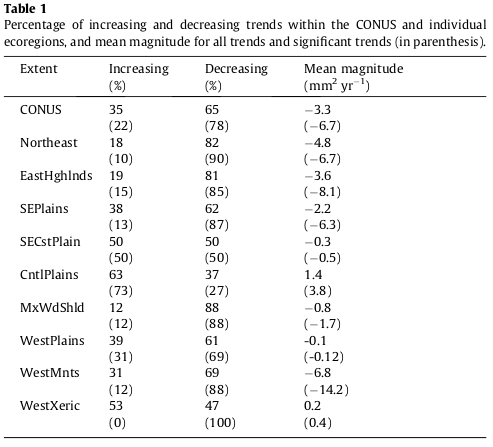
\includegraphics[width=.5\textwidth]{rice_streamflow_mean}
            \end{center}
    \end{enumerate}

\section{Lit. review: Maturity of topic}

    \begin{enumerate}
        \item Describe about how relativity new this subject is because of how dependent this index relies on GIS resolution
    \end{enumerate}

\section{Results: Goals? Findings?}

    \begin{enumerate}
        \item Mention that there seems to be a relationship between variables from Falcone 2016 "human distrubance" index and increased streamflow variability from Rice 2016
    \end{enumerate}

\section{Conclusion: (1/4) of paper. Summarize Conclusion}


    \begin{enumerate}
        \item The "human disturbance" index from Rice is a viable deductive approach to quantitativing human disturbance. 
        \item There is a relationship  between climatology and "human disturbance" index how they affect streamflow variability 
    \end{enumerate}

\section{References}


\end{document}
